\documentclass[12pt,border=5pt]{standalone}
\usepackage[utf8]{vietnam}
\usepackage{amsmath}
\usepackage{amsfonts} 
\usepackage{amssymb}
\usepackage{tikz}
\usetikzlibrary{calc}

\begin{document}

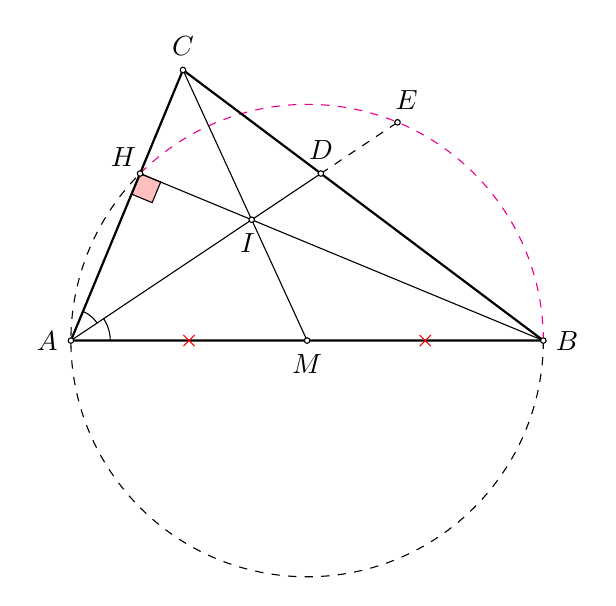
\begin{tikzpicture}
  [mark/.pic={\draw (45:.1)--(-135:.1) (-45:.1)--(135:.1);}]
  \def\a{3}
  \def\gH{135}
  \path
  (180:\a) coordinate (A)
  (0:\a) coordinate (B)
  (\gH:\a) coordinate (H)
  (0:0) coordinate (M)
  (\gH/2:\a) coordinate (E)
  (intersection of A--E and B--H) coordinate (I)
  (intersection of I--M and A--H) coordinate (C)
  (intersection of A--E and B--C) coordinate (D);
  % đánh dấu góc vuông H
  \draw[fill=pink,rotate=-\gH+22.5]
  (H) rectangle +(45:.4);
  \draw[dashed] (B) arc(0:\gH-360:\a) (D)--(E);
  \draw[dashed,magenta] (B) arc (0:\gH:\a);
  \draw (A)--(D) (C)--(M) (B)--(H);
  \draw[thick] (A)--(B)--(C)--cycle;
  \foreach \p in {A,B,C,D,M,H,E,I}
  \draw[fill=white] (\p) circle (1pt);
  \foreach \p/\g in {A/180,C/90,B/0,H/\gH,I/-100,D/90,E/.5*\gH,M/-90}
  \path (\p)+(\g:3mm) node{$\p$};
  % đánh đấu đoạn thẳng
  \path
  ($(A)!.5!(M)$) pic[red]{mark}
  ($(B)!.5!(M)$) pic[red]{mark};
  % đánh dấu các góc
  \begin{scope}
    \clip (B)--(A)--(D);
    \draw (A) circle(.5);
  \end{scope}
  \begin{scope}
    \clip (C)--(A)--(D);
    \draw (A) circle(.4);
  \end{scope}
\end{tikzpicture}

\end{document}